\section{Introduction}

Kernel matrices associated with the nonlinear feature map
of deep neural networks (NNs) provide insight into the optimization dynamics \citep{jacot2018neural,montanari2020interpolation,fort2020deep} and predictive performance \citep{lee2017deep,arora2019fine,ortiz2021can}; consequently, properties of these kernel matrices can guide the design of network architecture 
\citep{xiao2018dynamical,martens2021rapid,li2022neural} and learning algorithms
\citep{karakida2020understanding,zhou2022dataset}. Particular
emphasis has been placed on the \textit{spectral properties} of kernel matrices, due to their connection with the training and test performance of the underlying NN \citep{bordelon2020spectrum,loureiro2021learning,wei2022more}. 

In this paper, we focus on the \textit{conjugate kernel} (CK)
\citep{neal1995bayesian,cho2009kernel} defined as the Gram matrix of the
features at the penultimate (or more generally, any intermediate) NN layer.
In the high-dimensional asymptotic setting where the width of the NN and the
number of training samples diverge at the same rate, prior works 
employed random matrix theory to analyze the limit eigenvalue distribution of
the CK matrix at random initialization
\citep{pennington2017nonlinear,louart2018random,peche2019note,fan2020spectra}.
These and related characterizations of the CK resolvent enable precise
computations of various errors for NNs with random first-layer
weights, known as \textit{random features models} 
\citep{mei2019generalization,tripuraneni2021covariate,hassani2022curse}. 

It is worth noting that while existing results establish the weak convergence of
the empirical spectral measure, the precise behavior of ``spike'' eigenvalues
that are separated from the spectral bulk remains largely unexplored.
In learning applications, these spike eigenvalues and corresponding eigenvectors
are often the primary spectral features (signal) of interest, because they pertain to
low-rank structure of the underlying learning problem (e.g., class labels or
the direction of the target function). For the linearly defined \textit{spiked
covariance model} $\vX=\vZ\vSigma^{1/2} \in \R^{n \times d}$,
whose dependence across features is induced by a
linear map $\vSigma^{1/2}(\cdot)$ applied to $\vZ$ having i.i.d.\ coordinates,
classical work in random matrix theory provides a quantitative description of
the spike eigenvalue/eigenvector behavior
\citep{johnstone2001distribution,baik2006eigenvalues,benaych2012singular,bloemendal2016principal}.
In this paper, we establish an analogous characterization of spiked spectral
structure for the CK, motivated in part by the following applications: 

\begin{itemize}[leftmargin=*]
    \item \textbf{Structured input data.} Real data often contain low-dimensional structure despite the high ambient dimensionality \citep{lee2007nonlinear,hastie2009elements,pope2021intrinsic}, and the leading eigenvectors of the input covariance matrix may be good predictors of the training labels. 
    Common examples where the input features exhibit a low-dimensional spiked structure include
Gaussian mixture models \citep{loureiro2021learning,refinetti2021classifying,arous2023high1} and the
block-covariance setting of \citep{ghorbani2020neural,ba2023learning,mousavi2023gradient}. Assuming that the input data $\vX$ has informative spikes
eigenvectors, we ask the natural question: 
    \vspace{-1.mm}
    \begin{center}
        \textit{
        How does the low-dimensional signal propagate through nonlinear layers
of the NN? \\ When do we observe a similar spiked structure in the CK matrix? }
    \end{center}
    \item \textbf{Spiked weight matrices in early training.} It is known that NNs can
learn useful representations that adapt to the learning problem, and outperform
the random features model defined by randomly initialized weights \citep{ghorbani2019limitations,wei2019regularization,abbe2022merged}. 
    Recent works have shown that when the target function is low-dimensional,
the gradient update for two-layer NNs around initialization is \textit{low-rank}
\citep{ba2022high,damian2022neural,wang2022spectral}, and hence the updated weight matrix $\vW$
is well-approximated by a spiked model. We consider the following question on this pre-trained kernel model in NNs: 
    \vspace{-1.mm}
    \begin{center}
        \textit{
        When gradient descent produces a spiked structure in the weight matrix,
how does the feature representation of the NN change, in terms of spectral properties of the CK?}
    \end{center}
\end{itemize}

\subsection{Our Contributions}

We analyze the spike eigenstructure in a general nonlinear spiked 
covariance model, which includes the CK as a special case. Specifically, we
characterize the BBP phase transition \citep{baik2005phase} and first-order
limits of the eigenvalues and eigenvector alignments in the proportional
asymptotics regime, for spike eigenvalues of bounded size.
Our work makes the following contributions:
\begin{itemize}[leftmargin=*]
    \item \textbf{Signal propagation in deep random NNs.} Following the setup of
\cite{fan2020spectra}, we consider the CK matrix defined by a multi-layer
fully-connected NN at random initialization, where the width of each layer grows
linearly with the sample size. Given spiked input data, we compute the magnitude
of the leading CK eigenvalues and the alignments between the corresponding CK
eigenvectors with those of the input data, across network depth.
    \item \textbf{Feature learning in two-layer NNs.} We consider the
early-phase feature learning setting in \cite{ba2022high}, where the first-layer
weights in a two-layer NN are optimized by gradient descent, and the learned
weight matrix exhibits a rank-one spiked structure. We characterize the
spiked eigenstructure of the corresponding CK matrix for independent test data,
and the alignment of spike eigenvectors with the test labels.
This provides a quantitative description of how gradient descent improves the NN representation. 
    \item \textbf{Spectral analysis for nonlinear spiked covariance models.} We
give a general analysis of the signal eigenvalues/eigenvectors of spiked
covariance matrices with arbitrary and possibly nonlinear dependence across
features, showing a ``Gaussian equivalence'' with the quantitative spectral
properties of linear spiked covariance models established by
\cite{bai2012sample}. We prove a deterministic equivalent for the Stieltjes
transform and resolvent for any spectral argument separated from the support of
the limit spectral measure,
extending recent results for spectral arguments bounded away from the
positive real line \citep{chouard2022quantitative,chouard2023deterministic,schroder2023deterministic}.
\end{itemize}


\subsection{Related Works}

\paragraph{Eigenvalues of nonlinear random matrices.} 
Global convergence of the empirical eigenvalue distribution of
nonlinear kernel matrices has been studied in both proportional and polynomial
scaling regimes
\citep{el2010spectrum,cheng2013spectrum,fan2019spectral,lu2022equivalence,dubova2023universality}.
Building upon related techniques, recent works characterized the spectrum of the
CK matrix \citep{pennington2017nonlinear,louart2018random,peche2019note} and the
neural tangent kernel (NTK) matrix
\citep{montanari2020interpolation,adlam2020neural}, with generalizations to
deeper networks studied in \cite{fan2020spectra} and \cite{chouard2023deterministic}. 

\cite{benigni2022largest} gave a precise characterization
of the largest eigenvalue in a one-hidden-layer CK matrix when the input data
$\vX$ and weight matrix $\vW$ both have i.i.d.~entries, identifying possible
uninformative spike eigenvalues when the nonlinear activation is not an odd
function. \cite{guionnet2023spectral} and \cite{feldman2023spectral} recently
characterized spiked eigenstructure in models where an activation is applied to
a spiked Wigner matrix or rectangular information-plus-noise matrix entrywise,
for possibly growing spike sizes and activations having degenerate
information/Hermite coefficients.

\paragraph{Precise error analysis of NNs.} 
An important application of spectral analyses of the CK matrix is the precise
computation of generalization error of random features regression, 
first performed for two-layer models in proportional scaling regimes
\citep{louart2018random,mei2019generalization} and later extended to deep
random features models \citep{schroder2023deterministic,bosch2023precise} and
polynomial scaling regimes \citep{ghorbani2019linearized,xiao2022precise}. 
These risk analyses reveal a \textit{Gaussian equivalence principle}, where
generalization error coincides with that of a Gaussian covariates model,
and this equivalence has been extended to other settings of nonlinear
(regularized) empirical risk minimization 
\citep{hu2020universality,goldt2021gaussian,montanari2022universality}.

Going beyond random features, \cite{ba2022high} derived the
precise asymptotics of representation learning in a two-layer NN when the
first-layer weights are trained by one (or finitely many) gradient descent
steps; see also \cite{damian2022neural,ba2023learning,dandi2023learning}.
The computation follows from an information-plus-noise characterization
of the weight matrix due to a low-rank gradient update. \cite{moniri2023theory}
derived a corresponding information-plus-noise decomposition
of the CK matrix defined by the resulting trained weights, in an asymptotic
regime different from ours where the learning rate and spike eigenvalues
diverge. \cite{arous2023high2} examined the emerging spike
eigenstructure in the NN Hessian that arises during SGD training.

\paragraph{Eigenvalues of sample covariance matrices.} Asymptotic spectral
analyses of sample covariance matrices have a long history in random matrix
theory
\citep{marchenko1967,silverstein1995strong,silverstein1995empirical,bai1998no},
with the strongest known results in the linearly defined model
$\vX=\vZ\vSigma^{1/2}$, see e.g.\ \cite{bloemendal2014isotropic,knowles2017anisotropic}. Outside of this linear setting, \cite{srivastava2013covariance} and
\cite{chafai2018convergence} develop sharp bounds for the extremal eigenvalues
with isotropic population covariance, and \cite{bao2022extreme} develop
eigenvalue rigidity and Tracy-Widom fluctuation results for isotropic and log-concave distributions.

The spiked covariance model was introduced in \cite{johnstone2001distribution}.
\cite{baik2005phase,baik2006eigenvalues,paul2007asymptotics} initiated the study
of spiked eigenstructure and phase transition phenomena for spiked
covariance matrices with isotropic bulk covariance.
\cite{peche2006largest,benaych2011eigenvalues,benaych2012singular,capitaine2013additive,capitaine2018limiting}
studied spiked eigenstructure in related Wigner and information-plus-noise
models. Closely related to our work are the results of
\cite{bai2012sample} that characterize spike eigenvalues in linearly
defined models $\vX=\vZ\vSigma^{1/2}$ with general population covariance
$\vSigma$, and we extend this characterization to nonlinear settings.

\section{Results for neural network models}\label{sec:main_results}

\subsection{Propagation of signal through multi-layer neural networks}\label{sec:spike_CK}

Consider input features $\vX=[\vx_1,\ldots,\vx_n]\in\R^{d\times n}$, where
$\vx_i\in\R^d$ are independent samples. Define a $L$-hidden-layer feedforward neural network by
\begin{equation}\label{eq:NN}
    \vX_\ell=\frac{1}{\sqrt{d_\ell}}\sigma (\vW_\ell\vX_{\ell-1}) \in \R^{d_\ell
\times n} \qquad \text{ for } \ell=1\ldots,L
\end{equation}
with weight matrices $\vW_\ell \in \R^{d_\ell\times d_{\ell-1}}$, 
$\vX_0 \equiv \vX$ and $d_0 \equiv d$,
and a nonlinear activation function $\sigma:\R \to \R$ applied entrywise. The
Conjugate Kernel (CK) at each layer $\ell=1,\ldots,L$ is given by the Gram matrix
\begin{equation}\label{eq:K_L}
	\vK_\ell=\vX_\ell^\top\vX_\ell \in \R^{n \times n}.
\end{equation}

In the limit $n,d_0,\ldots,d_L \to \infty$ with
$n/d_\ell \to \gamma_\ell \in (0,\infty)$
for each $\ell=0,\ldots,L$, under deterministic
conditions for the input data $\vX$ and for random weight matrices
$\vW_1,\ldots,\vW_L$ as specified below, it is shown in \cite{fan2020spectra}
that the empirical eigenvalue distribution
$\widehat{\mu}_\ell$ of $\vK_\ell$ for each $\ell=1,\ldots,L$ satisfies
the weak convergence
\begin{equation}\label{eq:CKweakconvergence}
\widehat{\mu}_\ell:=\frac{1}{n}\sum_{i=1}^n \delta_{\lambda_i(\vK_\ell)}
\to \mu_\ell \text{ a.s.}
\end{equation}
for limit measures $\mu_1,\ldots,\mu_L$ defined 
as follows: Let $\mu_0$ be the limit eigenvalue distribution of the input gram
matrix $\vK_0=\vX^\top \vX$ (c.f.\ Assumption \ref{assump:data}).
Then, for $\ell=1,\ldots,L$, let
\begin{equation}\label{eq:nu_L_def}
	\nu_{\ell-1}=b_\sigma^2 \otimes \mu_{\ell-1} \oplus (1-b_\sigma^2)
\end{equation}
denote the law of $b_\sigma^2 \mathsf{x}+(1-b_\sigma^2)$ when $\mathsf{x}
\sim \mu_{\ell-1}$ and $b_\sigma:=\E_{\xi \sim \cN(0,1)}[\sigma'(\xi)]$,
and define
\begin{align}\label{eq:mu_L_def}
\mu_\ell=\rho^\MP_{\gamma_\ell}\boxtimes \nu_{\ell-1}.
\end{align}
Here, $\rho_\gamma^\MP \boxtimes \nu$ denotes the \emph{deformed Marcenko-Pastur
law} describing the limit eigenvalue distribution of a sample covariance
matrix with limit dimension ratio $\gamma \in (0,\infty)$ and population
spectral measure $\nu$, and we review its definition in Appendix
\ref{appendix:background}.

In this section, we provide a precise quantitative characterization of the spike
eigenvalues and eigenvectors of $\vK_\ell$ for each $\ell=1,\ldots,L$ when the
input data $\vX$ has a fixed number of spike singular values of bounded
magnitude. We assume the following conditions for the random weights, input
data, and activation.

\begin{assumption}\label{assump:NNasymptotics}
The number of layers $L \geq 1$ is fixed, and
$n,d_0,\ldots,d_L \to \infty$ such that
\[n/d_\ell \to \gamma_\ell \in (0,\infty) \text{ for each } \ell=0,\ldots,L.\]
The weights $\vW_1,\ldots,\vW_L$ have entries
$[\vW_\ell]_{ij} \overset{iid}{\sim} \cN(0,1)$, independent of each other and
of $\vX$.
\end{assumption}

\begin{defi}\label{def:ortho}
A feature matrix $\vX\in\R^{d\times n}$ is {\bf $\tau_n$-orthonormal} if
\[\big|\|\vx_{\alpha}\|_2-1\big| \leq \tau_n,
\qquad \big|\|\vx_{\beta}\|_2-1\big| \leq \tau_n,
\qquad \big|\vx_{\alpha}^\top \vx_{\beta}\big| \leq \tau_n\]
for all pairs $\alpha\neq \beta\in [n]$, where
$\{\vx_{\alpha}\}_{\alpha=1}^n$ are the columns of $\vX$.
\end{defi}

\begin{assumption}\label{assump:data}
For some $\tau_n>0$ such that $\lim_{n \to \infty} \tau_n \cdot n^{1/3}=0$,
$\vX \equiv \vX_0$ is $\tau_n$-orthonormal almost surely for all large $n$.
Furthermore, $\vK_0=\vX^\top \vX$ has eigenvalues
$\lambda_1(\vK_0),\ldots,\lambda_n(\vK_0)$
(not necessarily ordered by magnitude) such that
for some fixed $r \geq 0$, as $n,d \to \infty$,
\begin{enumerate}[label=(\alph*)]
\item There exists a compactly supported probability measure $\mu_0 $ on $[0,\infty)$ 
such that
$$\frac{1}{n-r}\sum_{i=r+1}^n \delta_{\lambda_i(\vK_0)} \to \mu_0
\text{ weakly a.s.}$$ 
and for any fixed $\eps>0$, almost surely for all large $n$,
\[\lambda_i(\vK_0) \in \supp{\mu_0}+(-\eps,\eps) \text{ for all }
i \geq r+1.\]   
\item  There exist distinct values $\lambda_1,\ldots,\lambda_r>0$ with
$\lambda_1,\ldots,\lambda_r \not\in\supp{\mu_0}$ such that
\[\lambda_i(\vK_0) \to \lambda_i\quad \text{ a.s.\ for each }\quad  i=1,\ldots,r.\]
\end{enumerate}
\end{assumption}

\begin{assumption}\label{assump:sigma}
The activation $\sigma:\R \to \R$ is twice differentiable with
$\sup_{x \in \R} |\sigma'(x)|,|\sigma''(x)| \leq \lambda_\sigma$
for some $\lambda_\sigma\in (0,\infty)$.
Under $\xi \sim \cN(0,1)$, we have
$\E[\sigma(\xi)]=0$ and $\E[\sigma^2(\xi)]=1$.
Furthermore,
\begin{equation}\label{eq:conditionsigma}
b_\sigma:=\E[\sigma'(\xi)] \neq 0, \qquad
\E[\sigma''(\xi)]=0.
\end{equation}
\end{assumption}

Assumption \ref{assump:NNasymptotics} defines the linear-width asymptotic
regime. Assumption \ref{assump:data} requires an orthogonality condition
for the input features that is similar to \cite[Definition 3.1]{fan2020spectra},
and also codifies our spiked eigenstructure assumption for the input data.
We briefly comment on \eqref{eq:conditionsigma}
in Assumption \ref{assump:sigma}: The condition $b_\sigma \neq 0$ ensures that
the linear component of $\sigma(\cdot)$ is non-degenerate; if $b_\sigma=0$,
then spiked eigenstructure does not propagate across the NN layers in our
studied regime of bounded spike magnitudes. The condition $\E[\sigma''(\xi)]=0$
ensures that $\vK_\ell$ does not have uninformative spike eigenvalues;
otherwise, as shown in \cite{benigni2022largest}, $\vK_\ell$ may have
spike eigenvalues even when the input $\vK_0$ has no spiked structure.
We assume $\E[\sigma''(\xi)]=0$ for clarity, to avoid characterizing also such
uninformative spikes across layers. This condition holds, in particular, for odd
activation functions $\sigma(\cdot)$ such as $\mathrm{tanh}$.

The following theorem first extends \cite[Theorem 3.4]{fan2020spectra} by
affirming that the weak convergence statement \eqref{eq:CKweakconvergence}
holds under the above assumptions, and furthermore, each $\vK_\ell$ has
no outlier eigenvalues outside its limit spectral support when the input
$\vK_0$ has no spike eigenvalues.

\begin{theorem}\label{thm:no_outlier_ck}
Suppose Assumptions \ref{assump:NNasymptotics}, \ref{assump:data},
and \ref{assump:sigma} hold. Then for each $\ell=1,\ldots,L$,
\eqref{eq:CKweakconvergence} holds weakly a.s.\ as $n \to \infty$. 
Furthermore, if the number of spikes is $r=0$ in Assumption \ref{assump:data},
then for any fixed $\eps>0$, almost surely for all large $n$,
\begin{align*}
\vK_\ell \text{ has no eigenvalues outside }
\supp{\mu_\ell}+(-\eps,\eps).
\end{align*}
\end{theorem}

The main result of this section characterizes the eigenvalues of $\vK_\ell$
outside $\supp{\mu_\ell}$ when $r\geq 1$. To describe this characterization,
define for each $\ell=1,\ldots,L$ the domain
\begin{align*}
\cT_\ell&=\{-1/\lambda:\lambda \in \supp{\nu_{\ell-1}}\}
\end{align*}
where $\nu_{\ell-1}$ is defined by \eqref{eq:nu_L_def},
and define $z_\ell,\varphi_\ell:(0,\infty) \setminus \cT_\ell \to \R$ by
\begin{align}
z_\ell(s)={-}\frac{1}{s}+\gamma_\ell \int\frac{\lambda}{1+\lambda s}
\nu_{\ell-1}(d\lambda), \qquad
\varphi_\ell(s)={-}\frac{sz_\ell'(s)}{z_\ell(s)}.
\label{eq:zell}
\end{align}
It is known from the results of \cite{bai2012sample} and
\cite[Chapter 11]{yao2015sample} that these are precisely the functions
that characterize the spike eigenvalues and eigenvectors in linear spiked
covariance models. Set
\[\cI_0=\{1,\ldots,r\}, \qquad
		s_{i,0}=-\frac{1}{b_\sigma^2\lambda_i+(1-b_\sigma^2)}
\text{ for } i \in \cI_0,\]
where $\lambda_i$ and $b_\sigma$ are defined in Assumptions~\ref{assump:data}
and~\ref{assump:sigma} respectively. Here, $\cI_0$ records the indices of the
spike eigenvalues of the input Gram matrix $\vK_0$.
Then define recursively for $\ell=1,\ldots,L$
\begin{equation}\label{eq:index_set}
\cI_\ell=\Big\{i \in \cI_{\ell-1}:z_\ell'(s_{i,{\ell-1}})>0\Big\},
\qquad
s_{i,\ell}=-\frac{1}{b_\sigma^2z_\ell(s_{i,{\ell-1}})+(1-b_\sigma^2)}
\text{ for } i \in \cI_\ell.
\end{equation}
The condition $z_\ell'(s_{i,\ell-1})>0$ describes the ``phase transition''
phenomenon for spike eigenvalues in this model, where spikes
$i \in \cI_{\ell-1}$ with
$z_\ell'(s_{i,\ell-1})>0$ induce spike eigenvalues in the CK matrix $\vK_\ell$
of the next layer, while spikes with $z_\ell'(s_{i,\ell-1}) \leq 0$ are
absorbed into the bulk spectrum of $\vK_\ell$.

 

\begin{theorem}\label{thm:ck_spike}
Suppose Assumptions~\ref{assump:NNasymptotics}, \ref{assump:data}, and
\ref{assump:sigma} hold.
Then for each $\ell=1,\ldots,L$:
\begin{enumerate}[label=(\alph*)]
\item $s_{i,\ell-1} \in (0,\infty) \setminus \cT_\ell$ for each $i \in \cI_{\ell-1}$,
so $z_\ell(s_{i,\ell-1})$ and $\cI_\ell$ are well-defined. Furthermore,
if $i \in \cI_\ell$ (i.e.\ if $z_\ell'(s_{i,\ell-1})>0$) then
$z_\ell(s_{i,\ell-1})>0$ and $\varphi_\ell(s_{i,\ell-1})>0$.
\item For any fixed and sufficiently small $\eps>0$, almost surely for all large $n$,
there is a 1-to-1 correspondence between the eigenvalues of $\vK_\ell$
outside $\supp{\mu_\ell}+(-\eps,\eps)$ and $\{i:i\in\cI_\ell\}$.
Denoting these eigenvalues of $\vK_\ell$ by
$\{\widehat \lambda_{i,\ell}:i\in\cI_\ell\}$,
for each $i\in \cI_\ell$ as $n \to \infty$,
\[\widehat \lambda_{i,\ell} \to z_\ell(s_{i,\ell-1}) \text{ a.s.}\]
\item Let $\widehat \vv_{i,\ell}$ be a
unit-norm eigenvector of $\vK_\ell$ corresponding to its eigenvalue
$\widehat \lambda_{i,\ell}$, and let $\vv_j$ be a
unit-norm eigenvector of $\vK_0$ corresponding to its spike
eigenvalue $\lambda_j(\vK_0)$.
Then for each $i \in \cI_\ell$ and $j \in \cI_0$, as $n \to \infty$,
	\[|\widehat \vv_{i,\ell}^\top \vv_j |^2 \to  \prod_{k=1}^\ell
\varphi_{k}(s_{i,k-1}) \cdot \bI\{i=j\} \text{ a.s.}\]
Moreover, for each $i \in \cI_\ell$ and any
unit vector $\vv\in\R^n$ independent of $\vW_1,\ldots,\vW_\ell$,
	\[|\widehat \vv_{i,\ell}^\top \vv |^2-\prod_{k=1}^\ell
\varphi_{k}(s_{i,k-1}) \cdot  |\vv_i^\top \vv |^2 \to 0 \text{ a.s.}\]
\end{enumerate}
\end{theorem}
\vspace{-4mm}
We present the following corollary as a concrete example in which the
assumptions of the theorem are satisfied. The corollary encompasses, for
instance, Gaussian mixture models with a fixed number $r$ of balanced classes,
each class having $\Theta(n)$ samples.
\begin{coro}\label{cor:gmm}
Suppose the input data $\vX$ is itself a low-rank signal-plus-noise matrix
\begin{equation}
	\label{eq:gmm}
\vX=\sum_{i=1}^r \theta_i\va_i\vb_i^\top+\vZ \in \R^{d\times n}
\end{equation}
where $\theta_1,\ldots,\theta_r>0$ are fixed distinct signal strengths,
$\va_1,\ldots,\va_r \in \R^d$ and $\vb_1,\ldots,\vb_r \in \R^n$ are
orthonormal sets of unit vectors, and
$\vZ$ has i.i.d.\ $\cN(0,1/d)$ entries. Assume that $\vb_1,\ldots,\vb_r$
satisfy the $\ell_\infty$-delocalization condition: for any sufficiently small
$\eps>0$ and all large $n$,
\[\max_{i=1}^r \|\vb_i\|_\infty<n^{-1/2+\eps}.\]
Define $\varphi_\ell(\cdot)$ and $s_{i,\ell-1}$ by \eqref{eq:zell}
and \eqref{eq:index_set}, with the initial measures $\mu_0=\rho_{\gamma_0}^\MP$
and $\nu_0=b_\sigma^2 \otimes \mu_0 \oplus (1-b_\sigma^2)$
and initial spike values
$\lambda_i=(1+\theta_i^2)(\gamma_0+\theta_i^2)/\theta_i^2$ for $i\in\cI_0$.

Then for each $\ell=1,\ldots,L$, $\vK_\ell$ has a spike eigenvalue corresponding
to the input signal component $\theta_i$ if and only if
$\theta_i>\gamma_0^{1/4}$ and $i \in \cI_\ell$. In this case,
its corresponding unit eigenvector $\widehat \vv_{i,\ell}$ satisfies, as $n \to
\infty$,
\begin{equation}\label{eq:gmmalignment}
|\widehat \vv_{i,\ell}^\top \vb_i|^2 \to
\prod_{k=1}^\ell \varphi_k(s_{i,k-1}) \cdot
\left(1-\frac{\gamma_0(1+\theta_i^2)}{\theta_i^2(\theta_i^2+\gamma_0)}\right)
\text{ a.s.}
\end{equation}
\end{coro}

\begin{figure}[t]
\centering
\begin{minipage}[t]{0.33\linewidth}
\centering
{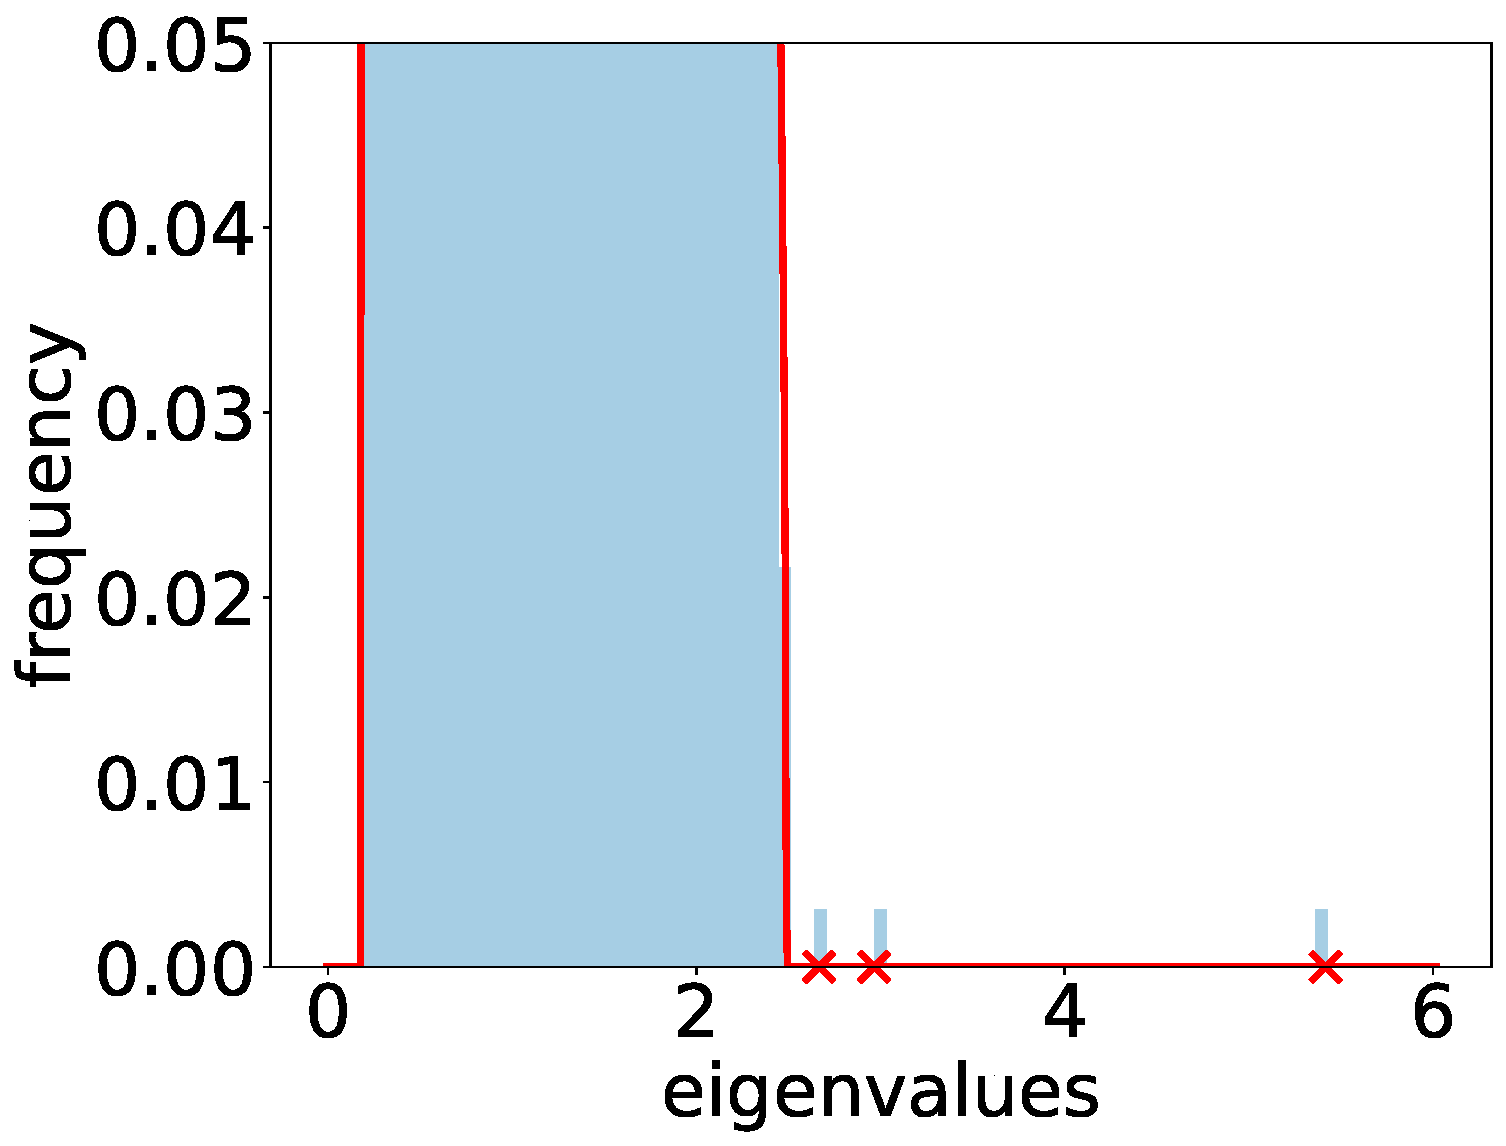
\includegraphics[width=\textwidth]{eigenvalues0.pdf}}  \\
\small (a) Spectrum of $\vK_0$ 
\end{minipage}%
\begin{minipage}[t]{0.33\linewidth}
\centering 
{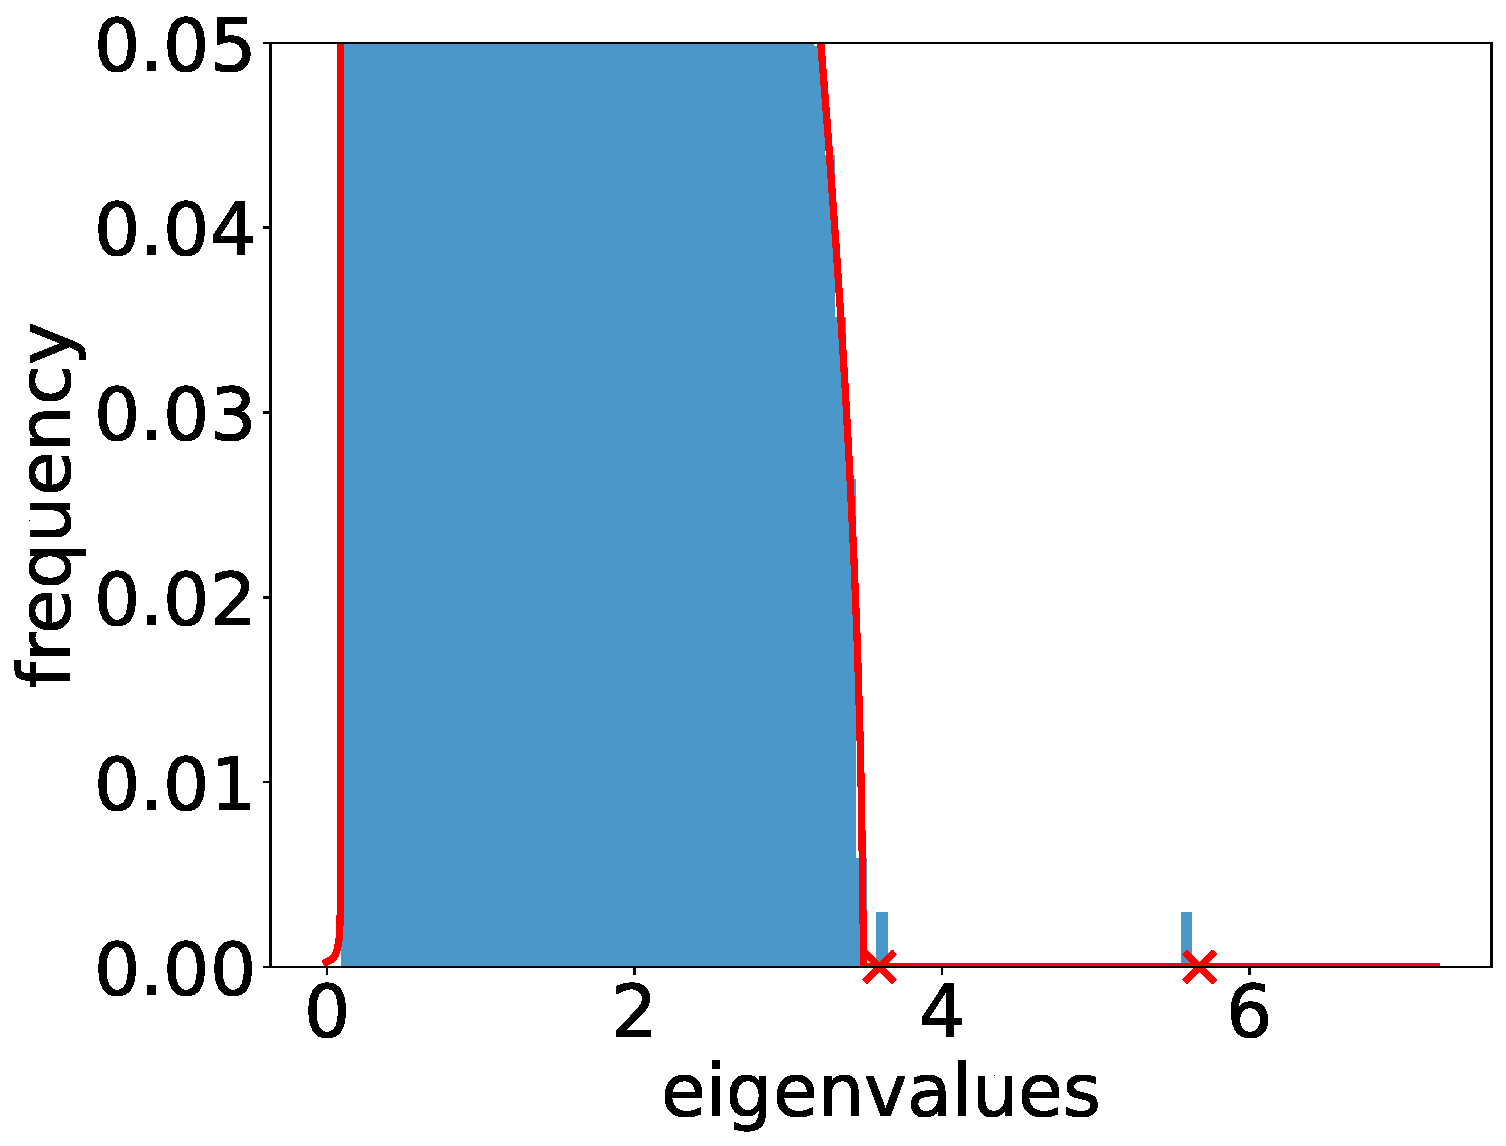
\includegraphics[width=\textwidth]{eigenvalues1.pdf}} \\ 
\small (b) Spectrum of $\vK_{1}$
\end{minipage}%
\begin{minipage}[t]{0.33\linewidth}
\centering 
{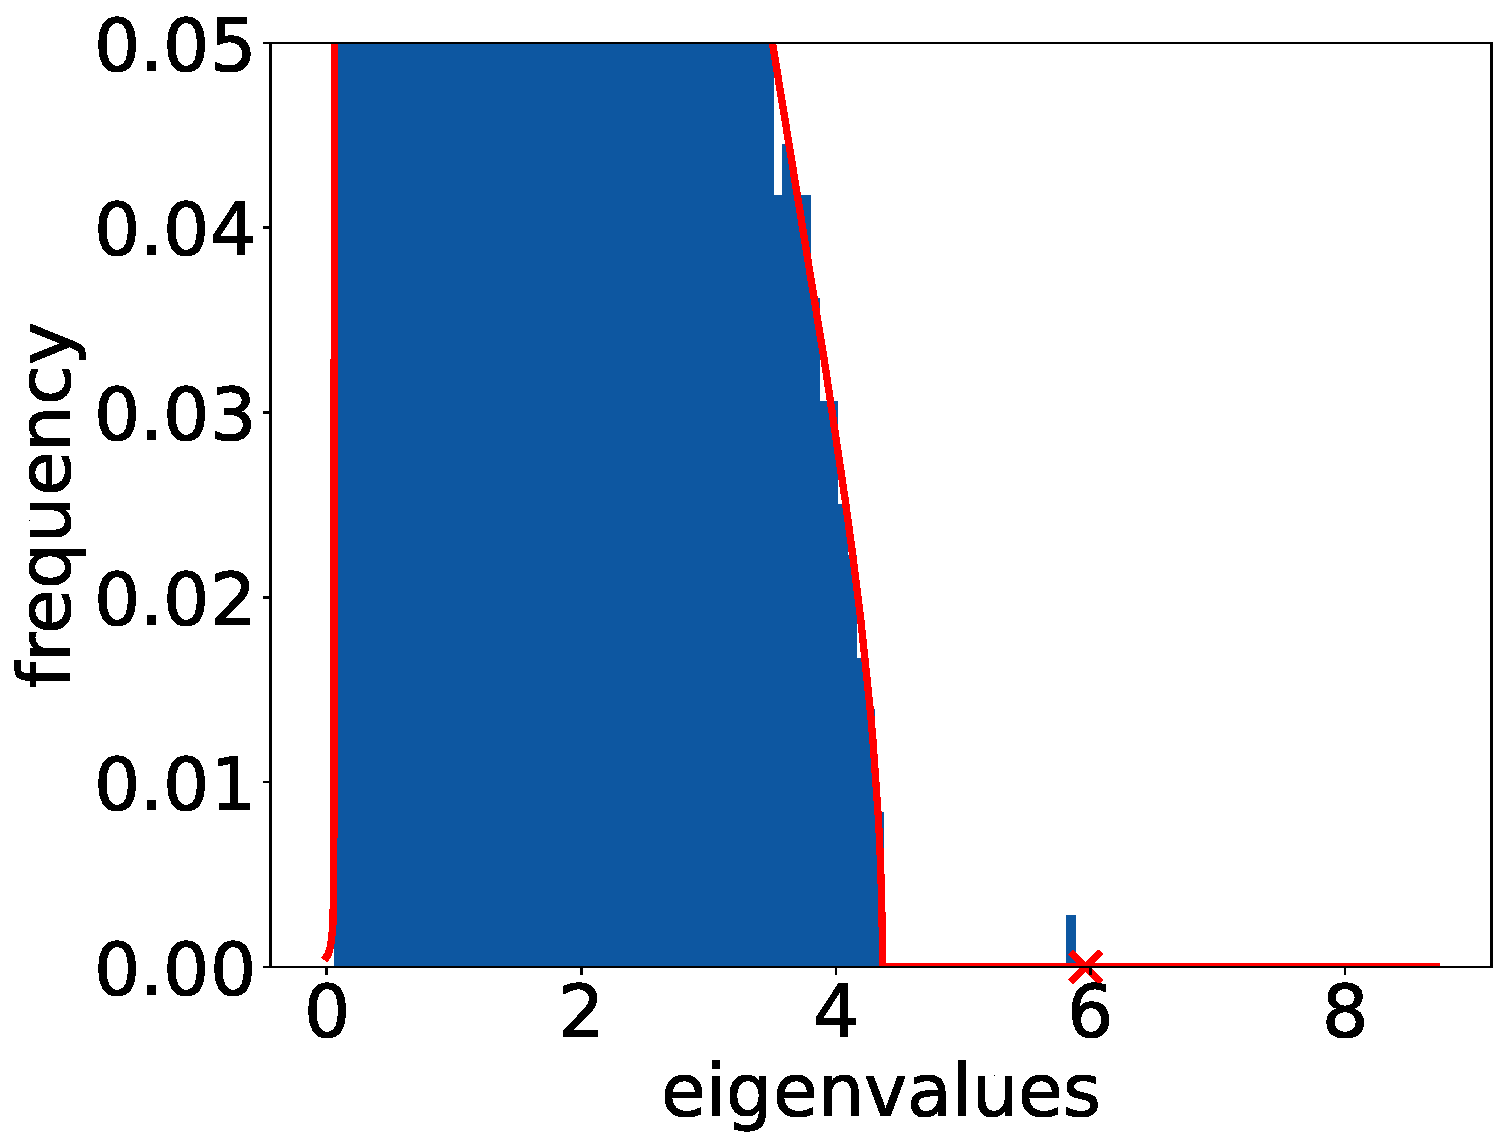
\includegraphics[width=\textwidth]{eigenvalues2.pdf}} \\ 
\small (c) Spectrum of $\vK_{2}$
\end{minipage}% 
\caption{\small  Spectra of three-layer CK matrices defined by \eqref{eq:K_L} with $n = 5000$,
$d_0=d_1=d_2 = 15000$, and $\sigma\propto \arctan$. Input data is a GMM satisfying \eqref{eq:gmm} with $r=3$, $\theta_1=2.0$, $\theta_2=1.18$,
and $\theta_3=1.0$. (a)-(c) are theoretically predicted (red) and empirical (blue)
bulk distributions and spikes of $\vK_\ell$ for $\ell=0,1,2$.}
\label{fig:GMM}  
\end{figure} 
\paragraph{Numerical illustration.}
A simple illustration of this result for a 3-component Gaussian mixture model
is provided in Figure \ref{fig:GMM}. We note that
$\cI_L \subseteq \cdots \subseteq \cI_0$ and $\varphi_\ell(s_{i,\ell-1})
\in (0,1)$, so the number of spike eigenvalues of $\vK_\ell$
induced by $\vK_0$ and the alignment of the spike eigenvectors of $\vK_\ell$
with the true class label vectors $\{\vb_i\}_{i=1}^r$ are both non-increasing in the network depth, see also Figure~\ref{fig:training}. In other words, at random initialization, the input signal diminishes as the depth of the NN increases. 

In Figure~\ref{fig:training} we highlight two remedies to this ``curse of depth'' at random initialization. 
\begin{itemize}[leftmargin=*]
    \item In Figure~\ref{fig:training}(a) we observe that when the width of NN becomes larger, alignment between the leading eigenvector of $\vK_\ell$ at random initialization and the signal can be preserved across a larger depth. This illustrates the benefit of overparameterization by increasing the network width. 
    \item In Figure~\ref{fig:training}(b) we observe that gradient descent training on the weight matrices also restores and even amplifies the informative signal in the CK matrix of each layer; specifically, after 50 steps of GD training (yellow curve), the alignment between the class labels and the leading eigenvector of $\vK_\ell$ may increase through depth. This demonstrates the benefit of gradient-based feature learning. In Section~\ref{sec:trained_CK} we precisely quantify this improved alignment due to gradient descent in a simplified two-layer setting. 
\end{itemize}

\begin{figure}[t]
\centering
\begin{minipage}[t]{0.42\linewidth}
\centering 
{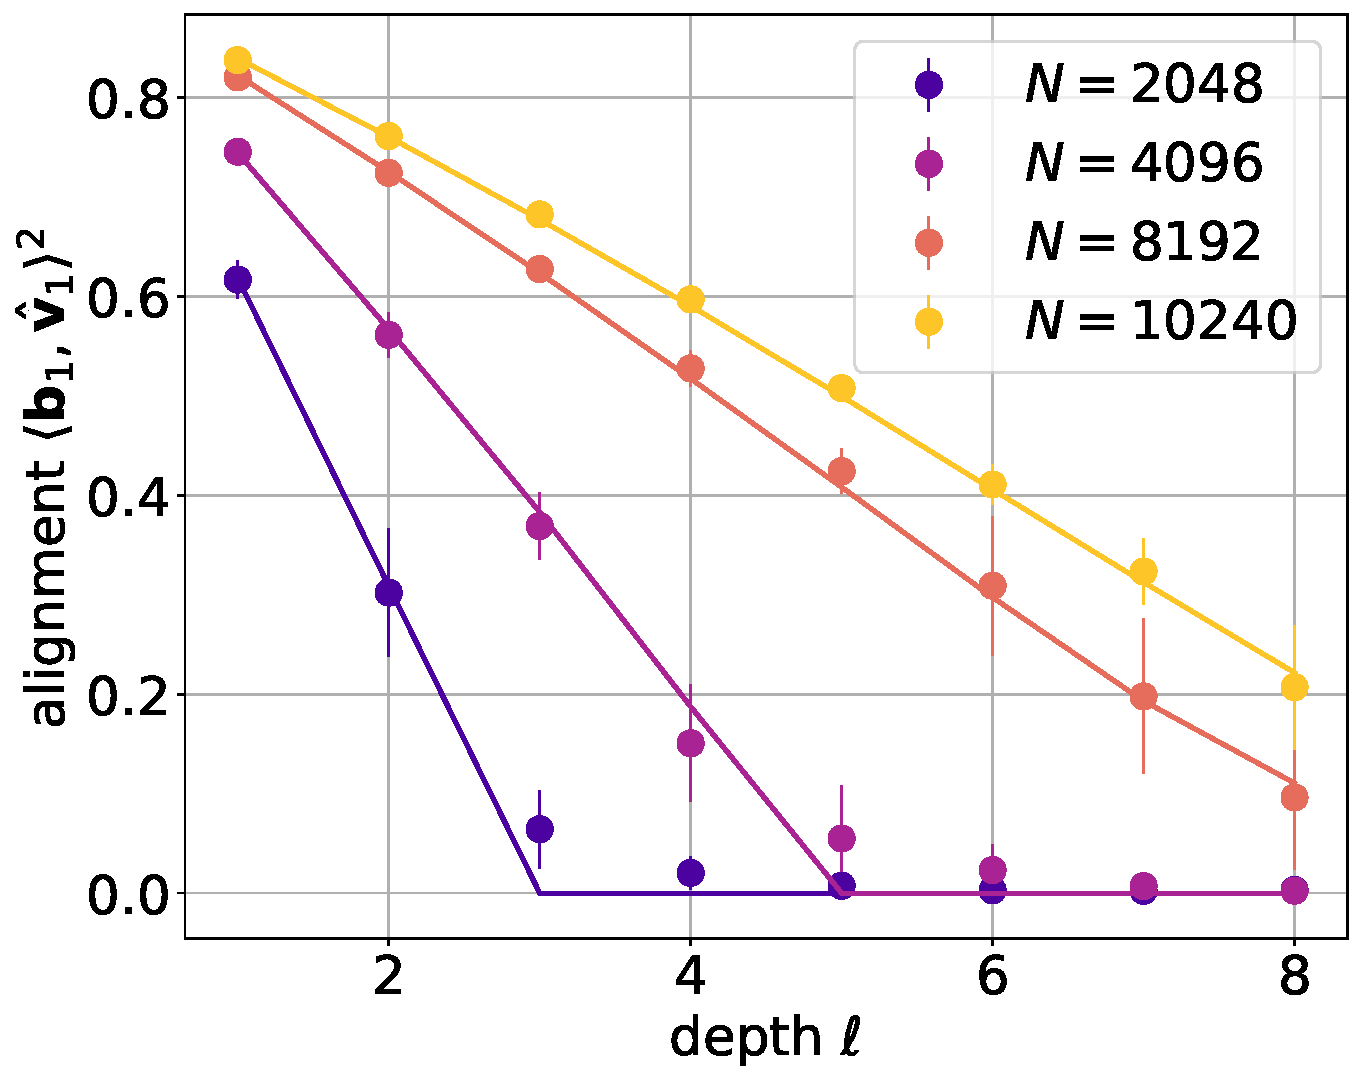
\includegraphics[width=0.8\textwidth]{alignment_vs_width.pdf}} \\ 
\small (a) Effect of width on alignment. 
\end{minipage}    
\begin{minipage}[t]{0.42\linewidth}
\centering
{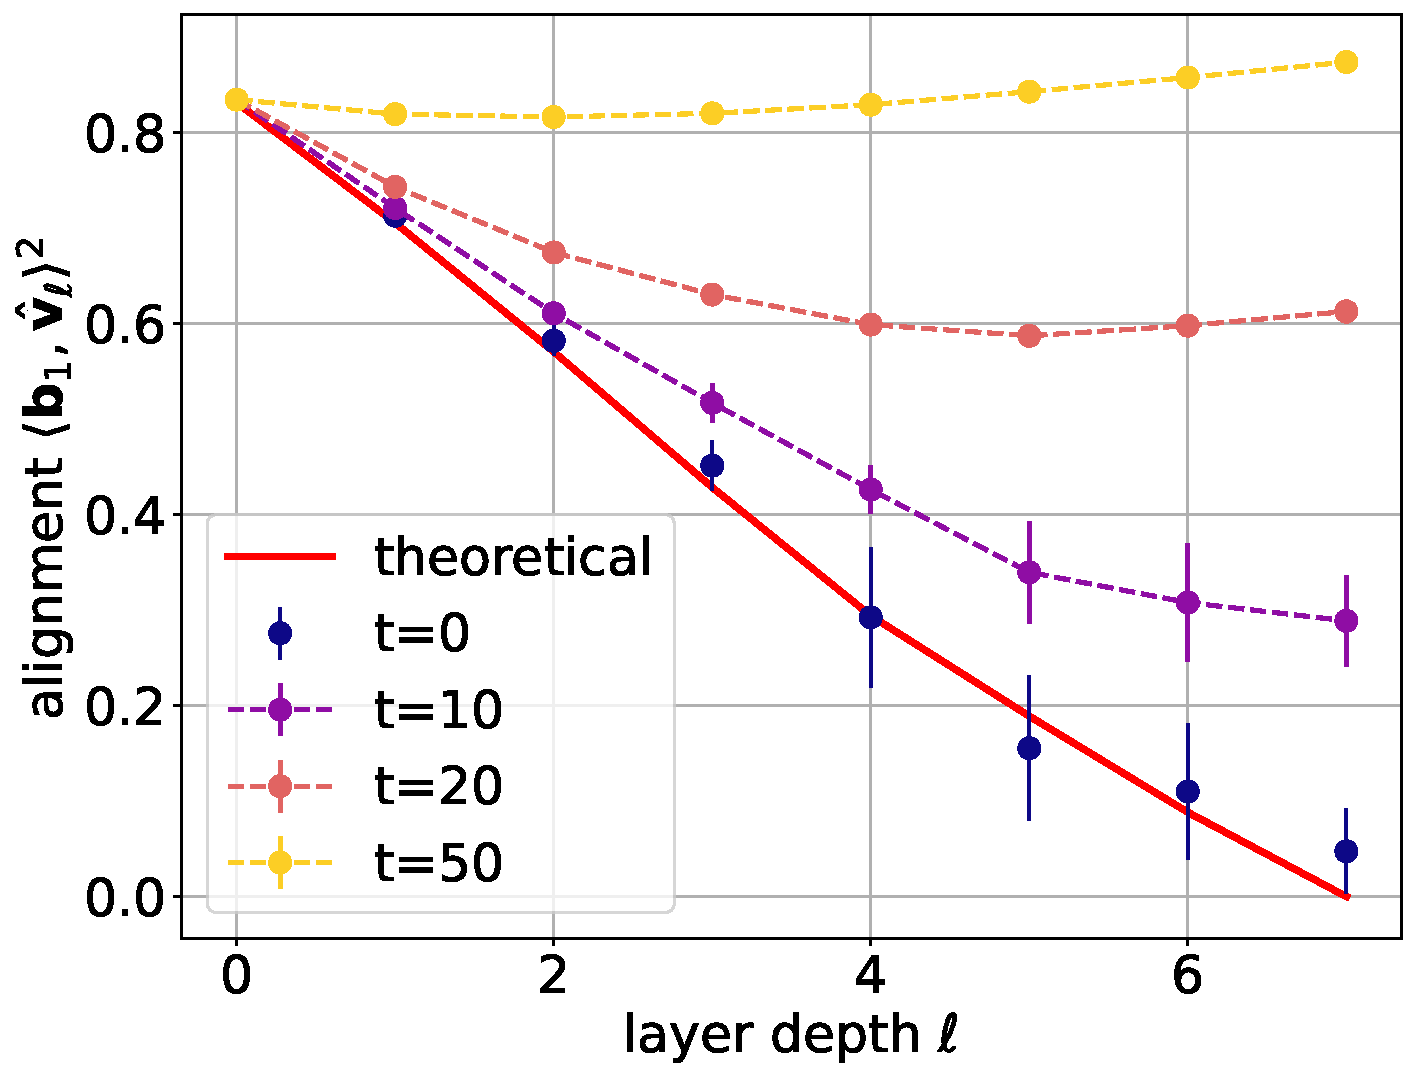
\includegraphics[width=0.83\textwidth]{trained_vs_init.pdf}}  \\
\small (b) Effect of GD training. 
\end{minipage} 
\caption{\small  We consider multiple-layer NNs in \eqref{eq:NN} with $ \sigma\propto \tanh$ on Gaussian mixture data \eqref{eq:gmm} for $r=1$, and compute the alignment between the largest eigenvector of the CK matrix $\vK_\ell$ with genuine signal $\vb_1$ (class labels) for different layer $\ell$. 
(a)  NNs at random initialization with varying hidden widths $N=2048,4096,8192,10240$. (b) NNs trained by gradient descent with learning rate $\eta=0.1$ for varying steps $T=0,10,20,50$; we use the $\mu$-parameterization \citep{yang2020feature} to encourage feature learning. $\theta_1$ is $2.5$ and  $1.8$ for (a) and (b), respectively. Dots are empirical values (over 10 runs) and solid curves represent theoretical predictions at random initialization from Theorem~\ref{thm:ck_spike}.  
}   
\label{fig:training}  
\end{figure}


\subsection{CK matrix after $O(1)$ steps of gradient descent}\label{sec:trained_CK}

The preceding section studied the spike eigenstructure of the CK induced by
low-rank structure in the input data.
Here, focusing on a two-layer model, we study an alternative setting 
where spiked structure arises instead
in the weight matrix $\vW$ from gradient descent training.

We consider an early training regime studied in \cite{ba2022high}, with
a width-$N$ two-layer feedforward NN,
\begin{align} 
f_{\text{NN}}(\vx)  
= \frac{1}{\sqrt{N}} \sum_{i=1}^N a_i\sigma(\langle \vx,\vw_i\rangle)
= \frac{1}{\sqrt{N}} \sigma(\vx^\top\vW)\va.
\label{eq:two-layer-nn}
\end{align} 
Here $\vx\in\R^d$ is the input, and
$\vW=[\vw_1,\ldots,\vw_N]\in\R^{d\times N}$ and $\va\in\R^N$ are the network
weights. For clarity of the subsequent discussion, we will
transpose the notation for $\vX$ and $\vW$ from the preceding section,
and incorporate a $1/\sqrt{d}$ scaling into $\vW$ rather than into the input
data $\vX$.

Given are an input feature matrix
$\vX=[\vx_1,\ldots,\vx_n]^\top \in \R^{n\times d}$ and labels $\vy \in \R^n$
for $n$ samples, where $y_i=f_*(\vx_i)+\text{noise}$.
We consider the training of first-layer weights $\vW$
to minimize the mean squared error
\[\cL(\vW) = {\frac{1}{2n}}\sum_{i=1}^n (f_{\text{NN}}(\vx_i)-y_i)^2,\]
fixing the second-layer weight vector $\va$.
From a random initialization $\vW_0 \in \R^{d \times N}$, and
over $T$ steps with learning rates $\eta_1,\ldots,\eta_T$ scaled by
$\sqrt{N}$, the gradient descent (GD) updates take the form
\begin{equation}\label{eq:trained_W}
	\vW_{\!t+1} = \vW_{\!t} + \eta_{t+1} \sqrt{N}\cdot\vG_t,
\qquad \vG_t=-\nabla\cL(\vW_t).
\end{equation}
Of interest is the information about the label function $f_*$ that is learned by
$\vW_{\text{trained}} \equiv \vW_T$, which may be characterized by the spectral
alignment of the CK matrix with the class label vector on independent
test data $(\tilde \vX,\tilde \vy)$.
This use of independent test data may be understood as a pre-training
setup, also considered previously
in \cite{ba2022high,moniri2023theory} and studied for real-world data in \cite{wei2022more}.

It was shown in \cite{ba2022high} that in a training regime
with initialization $\|\vW_0\| \asymp 1$ such that
$|f_{\text{NN}}(\vx_i)| \ll 1$ for each $i=1,\ldots,N$,
and with learning rates $\eta_1,\ldots,\eta_T \asymp
1$ for a fixed number $T$ of GD steps, the weight matrix $\vW$ undergoes a
change during training that is $O(1)$ in operator norm and approximately rank-1,
\[\vW_{\text{trained}}\approx \vW_0+\frac{\eta b_\sigma}{n}\vX^\top\vy\va^\top \qquad
\text{ where } \qquad \eta=\sum_{t=1}^T \eta_t.\]
Moreover, \cite[Conjecture 4]{ba2022high} conjectured that for the CK matrix
\begin{equation}\label{eq:trained_CK}
\vK=\frac{1}{N} \sigma(\tilde \vX\vW_{\text{trained}})\sigma(\tilde
\vX\vW_{\text{trained}})^\top \in \R^{n \times n}
\end{equation}
defined by the pre-trained weights and test data $\tilde \vX$,
the resulting spike eigenvalue and the alignment of its spike eigenvector with the test labels $\tilde
\vy \in \R^n$ are accurately predicted by a Gaussian equivalent model.
Our main result of this section is an affirmative verification of this
conjecture and precise characterization of the spike eigenstructure of $\vK$,
in the following representative setting.

\begin{assumption}\label{assum:GD}
For a two-layer NN in \eqref{eq:two-layer-nn} with GD training defined by \eqref{eq:trained_W}, we assume that~
\begin{enumerate}[label=(\alph*)]
\item $n,d,N \to \infty$ such that $N/d \to\gamma_0 \in
(0,\infty)$ and $N/n \to \gamma_1 \in (0,\infty)$. 
\item Training features $\vX=[\vx_1,\ldots,\vx_n]^\top \in \R^{n \times d}$
have entries $[\vX]_{ij} \overset{iid}{\sim} \cN(0,1)$, training labels $\vy \in
\R^n$ have entries
$y_i = \sigma_*(\vbeta_*^\top\vx_i)+\eps_i$ where $\vbeta_*\in\R^d$ is a
deterministic unit vector and
$\eps_i \overset{iid}{\sim} \cN(0,\sigma_\eps^2)$, and test data
$(\tilde \vX,\tilde \vy)$ is an independent copy of $(\vX,\vy)$.
\item The NN activation $\sigma:\R \to \R$ and label function
$\sigma_*:\R \to \R$ both satisfy Assumption~\ref{assump:sigma}, with
$b_\sigma:=\E[\sigma'(\xi)] \neq 0$ and
$b_{\sigma_*}:=\E[\sigma_*'(\xi)] \neq 0$.
\item The weight initializations satisfy
$[\vW_0]_{ij}\iid\cN(0,1/d)$ and $a_j \iid \cN(0,1/N)$.
\item The number of iterations $T$ and learning rates $\eta_1,\ldots,\eta_T$ are
fixed independently of $n,d,N$.
\end{enumerate}
\end{assumption}

Under these assumptions, the following theorem characterizes the spike eigenvalue of the CK matrix and the alignment between the corresponding eigenvector and the test labels, 
as a function of the learning rate $\eta_t$ and the number of gradient descent steps $T$. 

\begin{figure}[t]
\centering
\begin{minipage}[t]{0.46\linewidth}
\centering
{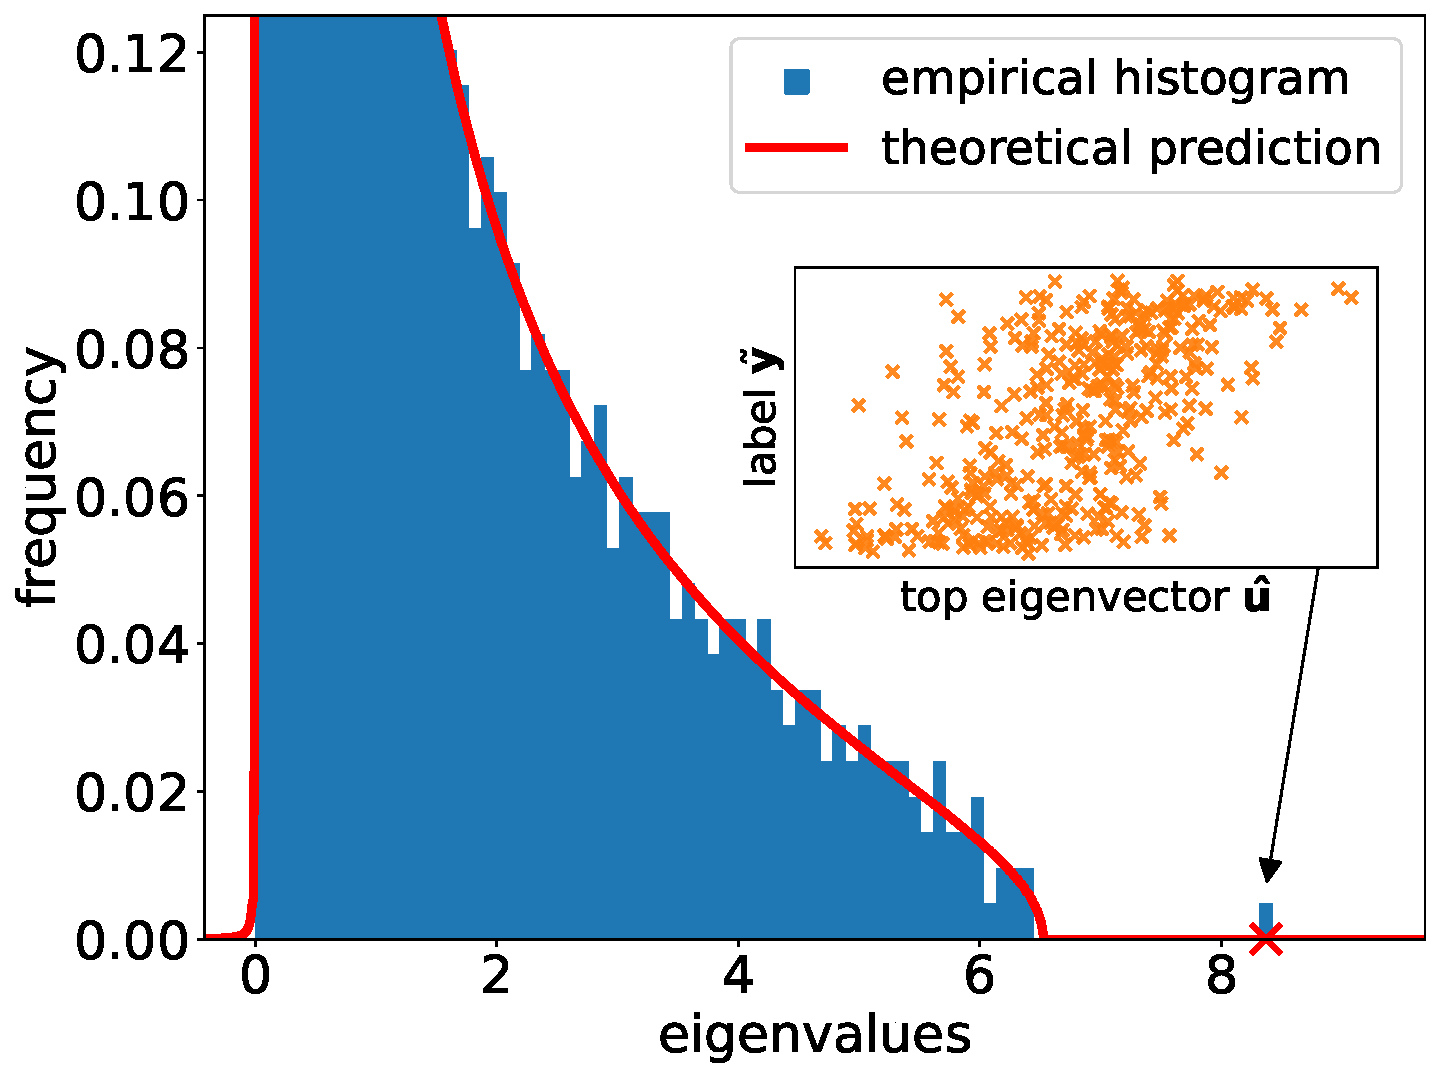
\includegraphics[height=0.6\textwidth]{GD_spike1.pdf}}  \\
\small (a) Spectrum of the updated CK. 
\end{minipage}
\begin{minipage}[t]{0.46\linewidth} 
\centering 
{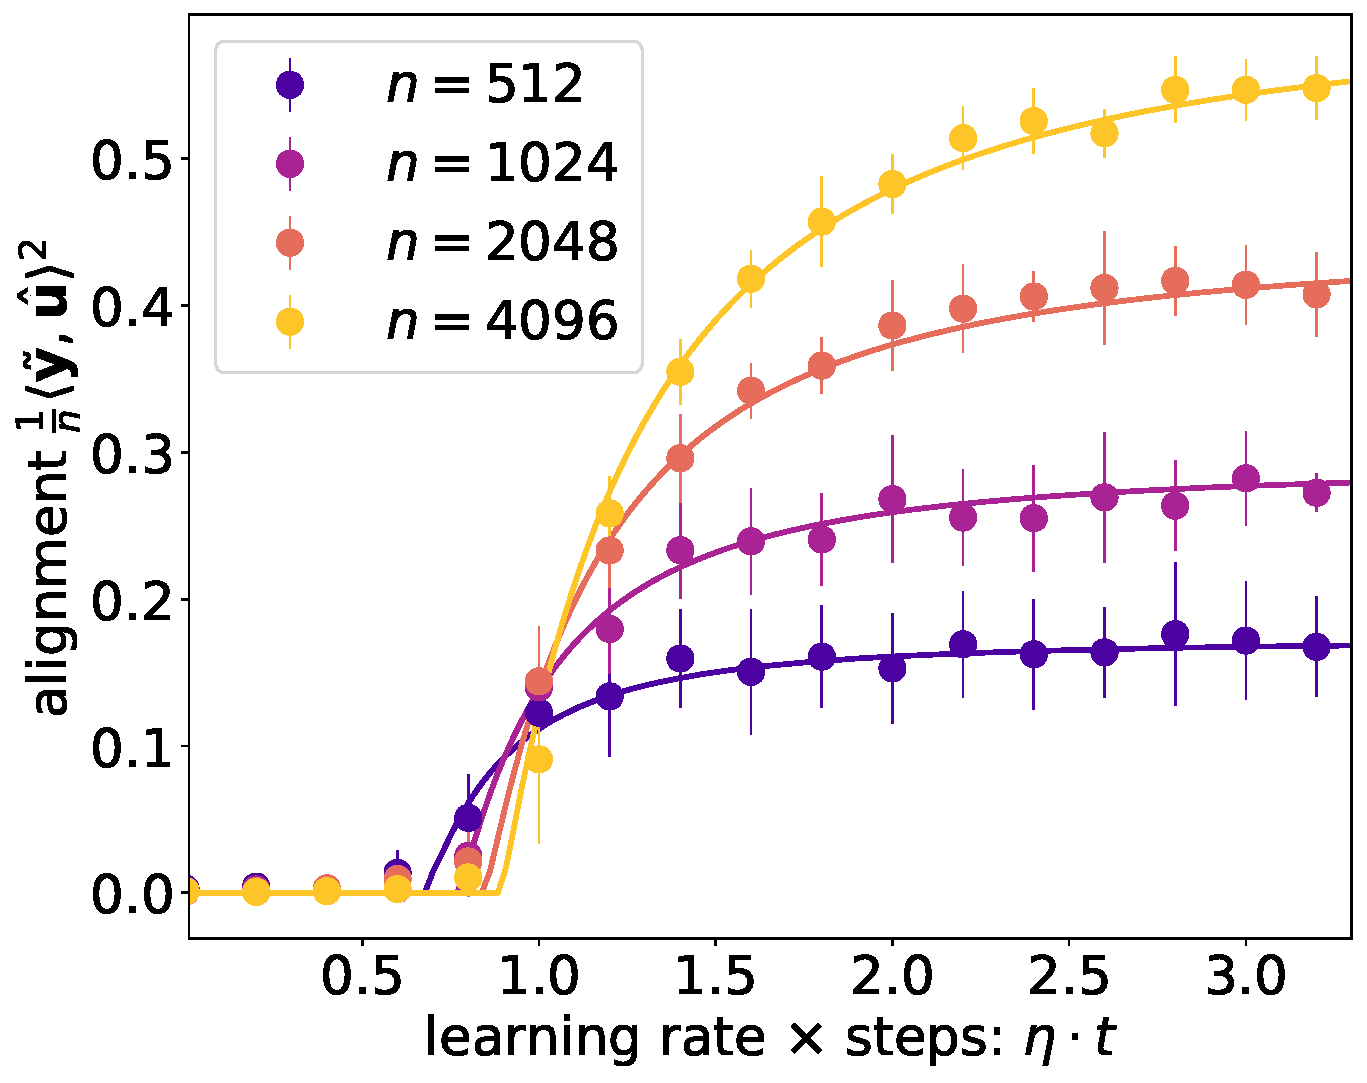
\includegraphics[height=0.6\textwidth]{GD_spike2.pdf}} \\ 
\small (b) Eigenvector alignment of the updated CK. 
\end{minipage}   
\caption{\small $(a)$ We set $n=2000, d=1600,N=2400,\eta\cdot t = 2$, and $\sigma=\sigma_*=\text{erf}$. 
$(b)$ We set $d=2048,N=1024,\eta=0.2$, $\sigma=\text{tanh}, \sigma_*=\text{SoftPlus}$, and vary the sample size $n$ and number of GD steps $t$; 
dots represent empirical simulations (over 10 runs) and solid curves are theoretical predictions from Theorem~\ref{thm:gd_spike}. 
 }   
\label{fig:GD}  
\end{figure} 

\begin{theorem}\label{thm:gd_spike}
Suppose that Assumption \ref{assum:GD} holds, and set
$\eta=\sum_{t=1}^T \eta_t$. Define  
\begin{equation}\label{def:theta_12}
\theta_1= b_\sigma\eta\cdot\sqrt{(\gamma_1/\gamma_0)(1+\sigma_\eps^2) +
b_{\sigma_*}^{2}}, \qquad
\theta_2=b_\sigma b_{\sigma_*}\eta.
\end{equation} 
Let $z_1(\cdot)$ and $\varphi_1(\cdot)$ be defined by \eqref{eq:zell} with
$\gamma_1$ and $\nu_0=b_\sigma^2\otimes\rho^{\MP}_{\gamma_0} \oplus (1-b_\sigma^2)$, and set
\[\lambda_1=b_\sigma^2\frac{(1+\theta_1^2)(\gamma_0+\theta_1^2)}{\theta_1^2}+1-b_\sigma^2.\]
Then $\vK$ defined by \eqref{eq:trained_CK} has a spike eigenvalue if and only
if $\theta_1>\gamma_0^{1/4}$ and $z'(-1/\lambda_1)>0$. In this case,
$\lambda_{\max}(\vK) \to \gamma_1^{-1}z(-1/\lambda_1)$ a.s.,
and the leading unit eigenvector $\widehat \vu\in\R^n$ of $\vK$ satisfies
\begin{equation}\label{eq:gd_alignment}
\frac{1}{\sqrt{n}}|\tilde{\vy}^\top \widehat\vu|\to b_\sigma b_{\sigma_*}
\frac{\sqrt{z(-1/\lambda_1)\varphi(-1/\lambda_1)}}{\lambda_1}\cdot
\frac{\theta_2\sqrt{(\theta_1^4-\gamma_0)(\gamma_0+\theta_1^2)}}{\theta_1^3}>0
\text{ a.s.}
\end{equation}
\end{theorem}

\paragraph{Numerical illustration.}
Figure~\ref{fig:GD} empirically validates the predictions of
Theorem~\ref{thm:gd_spike}, for a two-layer NN trained with a small number of
GD steps.
Figure \ref{fig:GD}(a) shows that one spike eigenvalue emerges over training in the test-data CK, the location of which is accurately predicted by Theorem~\ref{thm:gd_spike}; 
moreover, the leading eigenvector $\widehat{\vu}$ aligns with the labels $\tilde{\vy}$. 
This is quantified in Figure~\ref{fig:GD}(b), where above a phase transition
threshold, the alignment $\langle\widehat{\vu},\tilde{\vy}\rangle^2$ (predicted
by \eqref{eq:gd_alignment}) increases with the learning rate or number of GD steps; 
in addition, alignment also increases with the training set size $n$.
Compared with random initialization ($\eta=0$), this illustrates that training
improves the NN representation, and the test-data CK contains information on the label function $f_*$. 

\section{Analysis of a nonlinear spiked covariance model}\label{sec:proof_overview}

The results of Sections~\ref{sec:spike_CK} and~\ref{sec:trained_CK} rest on an
analysis of spiked eigenstructure in a general nonlinear spiked covariance
model. We describe the assumptions and statement of this general result
informally here, deferring formal and more quantitative statements
to Appendix \ref{sec:spiked_sample_covariance}.

Let
$\vG=\frac{1}{\sqrt{N}}[\vg_1,\ldots,\vg_N]^\top\in\R^{N\times n}$
have independent rows $\vg_1,\ldots,\vg_N \in \R^n$ with mean 0 and common
covariance $\vSigma \in \R^{n \times n}$. We assume that the law of $\vg_i$
satisfies concentration of quadratic forms $\vg_i^\top \vA\vg_j$, but has
otherwise arbitrary dependence across coordinates.
As $n,N \to \infty$ with $n/N \to \gamma \in (0,\infty)$,
the eigenvalues of $\vSigma$ satisfy
\[\lambda_i(\vSigma) \to \lambda_i \text{ for } i=1,\ldots,r, \qquad
\frac{1}{n-r}\sum_{i=r+1}^n \delta_{\lambda_i(\vSigma)} \to \nu \text{ weakly},\]
for fixed spike values $\lambda_1,\ldots,\lambda_r>0$ and a deterministic
limit spectral law $\nu$. Then the empirical spectral law of the sample
covariance matrix $\vK=\vG^\top \vG$ satisfies
\[\frac{1}{n}\sum_{i=1}^n \delta_{\lambda_i(\vK)} \to \mu=\rho_\gamma^{\MP}
\boxtimes \nu \text{ weakly a.s.}\]
Under these assumptions, let us define
\[z(s)={-}\frac{1}{m}+\gamma\int \frac{\lambda}{1+\lambda s}d\nu(\lambda),
\qquad \varphi(s)=\frac{z'(s)}{(-1/s)z(s)}.\]
\vspace{-\baselineskip}

\begin{theorem}[informal]\label{thm:informal}~
\begin{enumerate}[label=(\alph*)]
\item If $r=0$, then all eigenvalues of $\vK$ converge to
$\supp{\mu} \cup \{0\}$. More generally for $r \geq 0$, the eigenvalues of
$\vK$ asymptotically
separated from $\supp{\mu} \cup \{0\}$ are in 1-to-1 correspondence with
$\cI=\{i:z'(-1/\lambda_i)>0\}$, and
$\widehat{\lambda}_i(\vK) \to z(-1/\lambda_i)$.
\item For each $i \in \cI$ and any deterministic unit vector $\vv \in \R^n$,
$(\vv^\top \widehat \vv_i)^2-\varphi(-1/\lambda_i)(\vv^\top \vv_i)^2 \to 0$,
where $\vv_i,\widehat\vv_i$ are the unit eigenvectors of $\vSigma,\vK$ for
eigenvalues $\lambda_i(\vSigma),\widehat \lambda_i(\vK)$.
\item Let $\vu=\frac{1}{\sqrt{N}}(u_1,\ldots,u_N)^\top \in \R^N$ be such that
$[\vu,\vG] \in \R^{N \times (n+1)}$ has i.i.d.\ rows $\{[u_j,\vg_j]\}_{j=1}^N$, and denote
$\E[u\vg]=\E[u_j\vg_j]$ for all $j \in [N]$. Then for each $i \in \cI$,
\[(\vu^\top \widehat{\vu}_i)^2-\frac{z(-1/\lambda_i)\varphi(-1/\lambda_i)}{\lambda_i^2}
(\E[u\vg]^\top \vv_i)^2 \to 0\]
where $\widehat{\vu}_i$ is the unit eigenvector of
$\vG\vG^\top$ for its eigenvalue
$\widehat\lambda_i(\vG\vG^\top)=\widehat\lambda_i(\vK)$.
\end{enumerate}
\end{theorem}

Statements (a--b) are known in a linear
setting $\vg_i=\vSigma^{1/2}\vz_i$ when $\vz_i$ has i.i.d.\ entries,
see e.g.\ \citep{bai2012sample} and \cite[Theorems 11.3 and 11.5]{yao2015sample}. The above theorem thus
verifies an exact asymptotic equivalence between spiked spectral phenomena
in a nonlinear spiked covariance model with those of a linearly defined 
(possibly Gaussian) model.

In Section~\ref{sec:spike_CK}, each CK matrix $\vK_\ell$ has (approximately)
the structure of the above matrix $\vK$ over the randomness of $\vW_\ell$,
conditional on the features $\vX_{\ell-1}$ of the preceding layer, and
Theorem \ref{thm:ck_spike} follows from Theorem \ref{thm:informal}(a,b).
In Section~\ref{sec:trained_CK}, the CK matrix $\vK$ defined by trained weights
has (approximately) this structure over the randomness of $\tilde \vX$,
conditional on $\vW_{\mathrm{trained}}$, and Theorem
\ref{thm:gd_spike} follows from Theorem \ref{thm:informal}(a,c).

\paragraph{Proof ideas.} Analyses in the linearly defined model
$\vg_i=\vSigma^{1/2}\vz_i$ commonly stem from block matrix inversion identities 
with respect to the block decompositions
\[\vSigma=\begin{pmatrix}
	\vSigma_r & \mathbf{0}\\
	\mathbf{0} & \vSigma_0
\end{pmatrix}, \qquad
\vG=\begin{pmatrix} \vG_r & \vG_0 \end{pmatrix}\]
where $\vSigma_r$ contains the spike eigenvalues of $\vSigma$, and $\vG_r$ is
independent of $\vG_0$. This independence does not hold in our setting,
and we develop a different ``master equation'' approach.

Let $\widehat\lambda^{1/2}$ be a spike singular value of $\vG$ with
corresponding unit singular vectors $(\widehat\vu,\widehat\vv)$. We consider the
linearized equation
\begin{equation}\label{eq:linearized}
0=\begin{pmatrix} -\widehat{\lambda}\vI & \vG^\top \\ \vG & -\vI \end{pmatrix}
\begin{pmatrix} \widehat\vv \\ \widehat{\lambda}^{1/2}\widehat\vu
\end{pmatrix}.\end{equation}
Writing $\vV_r \in \R^{n \times r}$ for the $r$ spike eigenvectors of $\vSigma$,
we define a generalized resolvent
\[\vcR(z,\alpha)=\begin{pmatrix} -z\vI-\alpha\vV_r\vV_r^\top & \vG^\top \\ \vG & -\vI
\end{pmatrix}^{-1},\]
add to \eqref{eq:linearized} the quantity
$-\alpha \begin{pmatrix} \vV_r \\ \mathbf{0}
\end{pmatrix} \cdot \vV_r^\top \widehat \vv$ on both sides for some large
$\alpha>0$, and rewrite this as
\begin{equation} \label{eq:eigenvector_master}
\begin{pmatrix} \widehat\vv \\ \widehat\lambda^{1/2}\widehat\vu \end{pmatrix}
=-\alpha\,\vcR(\widehat\lambda,\alpha)\begin{pmatrix}\vV_r \\ \mathbf{0} \end{pmatrix}
\cdot \vV_r^\top \widehat\vv.
\end{equation}
We will show that $\vcR(z,\alpha)$ exists and is bounded in operator norm
for any $z$ separated from the limit
bulk spectral support of $\vK$ and any large enough $\alpha>0$. Then,
multiplying \eqref{eq:eigenvector_master} by $(\vV_r^\top\;\mathbf{0})$ and
applying a block matrix inversion identity,
\begin{align*}
\vV_r^\top \widehat\vv&={-}\alpha \begin{pmatrix} \vV_r \\ \mathbf{0}
\end{pmatrix}^\top \vcR(\widehat\lambda,\alpha)\begin{pmatrix}\vV_r \\ \mathbf{0} \end{pmatrix}
\cdot \vV_r^\top \widehat\vv
=-\alpha \vV_r^\top\Big(\vG^\top
\vG-\widehat\lambda \vI-\alpha\vV_r\vV_r^\top \Big)^{-1}\vV_r \cdot \vV_r^\top \widehat\vv.
\end{align*}
As a result, spike eigenvalues $\widehat\lambda$ are roots
$z=\widehat\lambda$ of the master equation
	\[\det\left(\vI_{r}+\alpha
\vV_r^\top\Big(\vG^\top\vG-z\vI-\alpha\vV_r\vV_r^\top\Big)^{-1}\vV_r \right)=0,\]
for any fixed and large $\alpha>0$. Singular vector alignments may be
characterized likewise from \eqref{eq:eigenvector_master}.

The core of the proof is an asymptotic analysis of this master equation
via a deterministic equivalent approximation
\begin{equation}\label{eq:detequivinformal}
\vv_1^\top \vR(\vGamma)\vv_2:=
\vv_1^\top (\vG^\top \vG-\vGamma)^{-1}\vv_2 \approx {-}\vv_1^\top
(\vGamma+z\tilde m(z)\vSigma)^{-1}\vv_2
\end{equation}
for any deterministic unit vectors $\vv_1,\vv_2 \in \R^n$ and low-rank perturbations $\vGamma$
of $z\vI$, where $\tilde m(z)$ is the
Stieltjes transform of the ``companion'' limit measure $\tilde \mu$ for the
eigenvalue distribution of $\vG\vG^\top \in \R^{N \times N}$. We extend
results of \cite{chouard2022quantitative,schroder2023deterministic}
by establishing this approximation not only for $\vGamma=z\vI$ but also
perturbations thereof, and for spectral arguments $z \in \C \setminus
\supp{\mu}$ that may belong to the positive real line. The latter
extension requires showing, a priori, that all eigenvalues of
$\vK=\vG^\top \vG$ fall close to $\supp{\mu}$ in the absence of spiked structure.
We show this by adapting an argument of \cite{bai1998no} and using a fluctuation
averaging lemma described below.

Let us conclude with a brief discussion of our proof
of \eqref{eq:detequivinformal}: From manipulations of the identity
	\[\Tr \vB=
\Tr (\vG^\top \vG-\vGamma)\vR(\vGamma)\vB={-}\Tr
\vR(\vGamma)\vB\vGamma+\frac{1}{N}\sum_{i=1}^N \vg_i^\top \vR(\vGamma)\vB\vg_i\]
for appropriately chosen matrices $\vB \in \C^{n \times n}$,
the Sherman-Morrison (leave-one-out) formula for matrix
inversion applied to $\vR(\vGamma)$, and the concentration of bilinear
forms in $\vg_i$, one may show
\begin{equation}\label{eq:prefluctavg}
\vv_1^\top (\vGamma+z\tilde m(z)\vSigma)^{-1}\vv_2
\approx {-}\vv_1^\top \vR(\vGamma)\vv_2+
			 \frac{1}{1+N^{-1}\Tr \vSigma\vR(\vGamma)}
			 \cdot \frac{1}{N}\sum_{i=1}^N (1-\E_{\vg_i})T_i
\end{equation}
where $T_i=\vg_i^\top
	\vR^{(i)}(\vGamma)\vv_2 \cdot \vv_1^\top(\vGamma+z m_{\tilde
\vK}^{(i)}(\vGamma)\vSigma)^{-1} \vg_i$. Here, $\vR^{(i)}(\vGamma)$ and
$m_{\tilde \vK}^{(i)}(\vGamma)$ are generalized leave-one-out resolvents and
empirical Stieltjes transforms defined by $\{\vg_j\}_{j \neq i}$, and $\E_{\vg_i}$
is the partial expectation over only $\vg_i$. Under our assumptions for $\vg_i$,
each error term $(1-\E_{\vg_i})T_i$ has mean 0 and $O(1)$ fluctuations.
We develop a fluctuation averaging lemma using recursive applications of the
Sherman-Morrison identity to further resolve the dependence of
$\vR^{(i)}(\vGamma)$ and $m_{\tilde \vK}^{(i)}(\vGamma)$ on fixed subsets of
rows $\{\vg_j\}_{j \neq i}$, to show that the errors
$(1-\E_{\vg_i})T_i$ are weakly correlated across $i \in [N]$. Hence their
average has a mean 0 and fluctuates on the asymptotically negligible
scale of $O(N^{-1/2})$, and applying this to \eqref{eq:prefluctavg} shows
\eqref{eq:detequivinformal}.


\bigskip

